In this section, we define the attacker model and show the security guarantees given by \lang. Specifically, we show that \lang{} executions satisfy termination-insensitive noninterference (TINI) \cite{4223226}. Formally, an attacker is some principal $\Attacker$. Note that this principal might be a conjunction of named principals $n_1 \wedge \dots \wedge n_k$ representing a set of $k$ colluding principals. In the sections that follow we denote a $\Nameset$-indexed set of stores as a function $\globalstore: \Nameset \to (\Addr \partialto \val)$.

\subsection{Trace semantics}
We express the attacker model in terms of a trace semantics, in which certain operations in the language emit \emph{events} which may or may not be observable by $\Attacker$. The grammar for events is given in Figure~\ref{fig:event-syntax}. These events should be self-explanatory, except for $\mathsf{release}$ events, which we explain later in this section. A non-empty event $\event$ contains the type of the event, the current environment when the event was emitted, and the node that emitted the event. An attacker observes modifications to memory (i.e., writes or allocations) locally on a node and remote procedure calls and returns across nodes.

\begin{figure}
\centering
\begin{align*}
\event &::= (\alpha, \env, n) \mid \varepsilon\\
\alpha &::= \mathsf{write}(\addr, \expr) \mid \mathsf{new}(\addr, \expr) \mid \mathsf{call}(\expr, n) \\ &\quad \mid \mathsf{ret}(\val, n) \mid \mathsf{stop}(\val, n) \mid \mathsf{release}(p, q, r)
\end{align*}
\caption{The syntax of events.}
\label{fig:event-syntax}
\end{figure}

We call a sequence of events a \emph{trace}. We write the concatenation of traces as $t_1 \cdot t_2$ and we write the empty trace as $\varepsilon$. Given a trace $t$ the observable trace of $t$ is the trace $t \upharpoonright \Attacker$, defined as
\begin{align*}
\varepsilon \upharpoonright \Attacker &= \varepsilon\\
((\alpha, \env, n) \cdot t) \upharpoonright \Attacker &=
\begin{cases}
(\alpha, \env, n) \cdot (t \upharpoonright \Attacker) & \nopostflowstoquery{n; \env}{\env_n.\lblkw}{\Attacker} \\
t \upharpoonright \Attacker & \text{otherwise}
\end{cases}
\end{align*}
We augment the semantics from Section~\ref{sec:calculus} with events. Figure~\ref{fig:event-semantics} shows an excerpt of the augmented semantics (we use $[\ldots]$ to elide the premises presented in Section~\ref{sec:calculus}). Except for the emitted event these rules correspond exactly to the rules in Figure~\ref{fig:monadic-reductions} and Figure~\ref{fig:global-steps}. We write $\gconfig{n}{\env}{S} \gstepstos[][t]$ when there exists a configuration $\gconfig{n'}{\env'}{S'}$ such that $\gconfig{n}{\env}{S} \gstepstos[][t] \gconfig{n'}{\env'}{S'}$ and $\termsym(S'_n)$ for all $n$. We also write $\gconfig{n}{\env}{S} \gstepstos[][\Attacker \filtertrace t']$ when $\gconfig{n}{\env}{S} \gstepstos[][t]$ and $t' = \Attacker \upharpoonright t$.

\begin{figure}
\centering
\begin{mathpar}
\inferrule[E-Write-Ev]{[\ldots] \and \event = (\mathsf{write}(\addr, \expr'), \env, n)}{\step{n; \env}[][\event]{\config{\store}{\efill{\writeref{\addr}{\expr'}}}}{ \config{\store'}{\efill{\return{()}}}}{\sigma}}
\and
\inferrule[G-Step-Ret-Ev]{S_n = \config{\store_n}{\efill{\wait{m}[\type]}} \and S_m = \config{\store_m}{\val ; \overline{\expr_m}} \\\\ \event = (\mathsf{ret}(\val, n), \env, m)}{\gconfig{m}{\env}{S} \gstepsto[][\event] \gconfig{n}{\env}{\extends{S}{n \mapsto \config{\store_n}{\efill{\val}}, m \mapsto \config{\store_m}{\overline{\expr_m}}}}}
\and
\inferrule[G-Step-Local-Ev]{\step{n; \env}[][\event]{S_n}{s}{\sigma}}{\gconfig{n}{\env}{S} \gstepsto[][\event] \gconfig{n}{\extend{\env}{n}{\sigma}}{\extend{S}{n}{s}}}
\and
\inferrule[E-Assume-Ev]{
[\ldots] \and \event = (\mathsf{release}(p, q, r), \env, n)}{\step{n; \env}[][\event]{\config{\store}{\efill{\adddelegate{p}{q}{r}}}}{ \config{\store}{\efill{\return{()}}}}{\sigma}}
\end{mathpar}
\caption{Augmented semantics emitting events.}
\label{fig:event-semantics}
\end{figure}

\paragraph{Release events}\label{sec:release-events}
To define noninterference, we require that nodes agree on which principals flow to $\Attacker$. That is, it must \emph{not} be the case that $\mathsf{Alice}$ considers data to not be observable by $\Attacker$, and then send it to $\mathsf{Bob}$, who considers the same data to be observable by $\Attacker$. Relaxations of such limitations, like robust declassification \cite{Zdancewic:2001:RD:872752.873524, Myers:2004:ERD:1009380.1009673} and nonmalleable information-flow \cite{Cecchetti:2017:NIF:3133956.3134054}, is orthogonal to this work and we consider only the case where nodes agree on which principals flow to $\Attacker$ in the information-flow lattice. To capture this intuition, we introduce the notion of a \emph{good} release event. Intuitively, when only good events are emitted the nodes agrees on what information flows to $\Attacker$.

\paragraph{Good events}
We call a release event $\event = (\mathsf{release}(p, q, r), \env, n)$ good, written $\good{\Attacker}{\event}$, if $\nopostflowstoquery{n; \env}{r}{\Attacker}$ implies $\nopostflowstoquery{n; \env}{p}{\Attacker} \iff \nopostflowstoquery{n; \env}{q}{\Attacker}$. Intuitively, this means that any expression of the form $\adddelegate{p}{q}{r}$ such that $r$ flows to $\Attacker$ should not modify what the attacker can observe. An illustration capturing when a flow is not good is shown in Figure~\ref{fig:bad-release}. We extend the notion of good to traces and say a trace is good, written $\good{\Attacker}{t}$ if all release events in $t$ are good release events. Our noninterference result, presented at the end of this section, will quantify only over good traces, and we leave the problem of extending this result to more relaxed notions of noninterference as future work.

\begin{figure}
\begin{minipage}{0.25\textwidth}
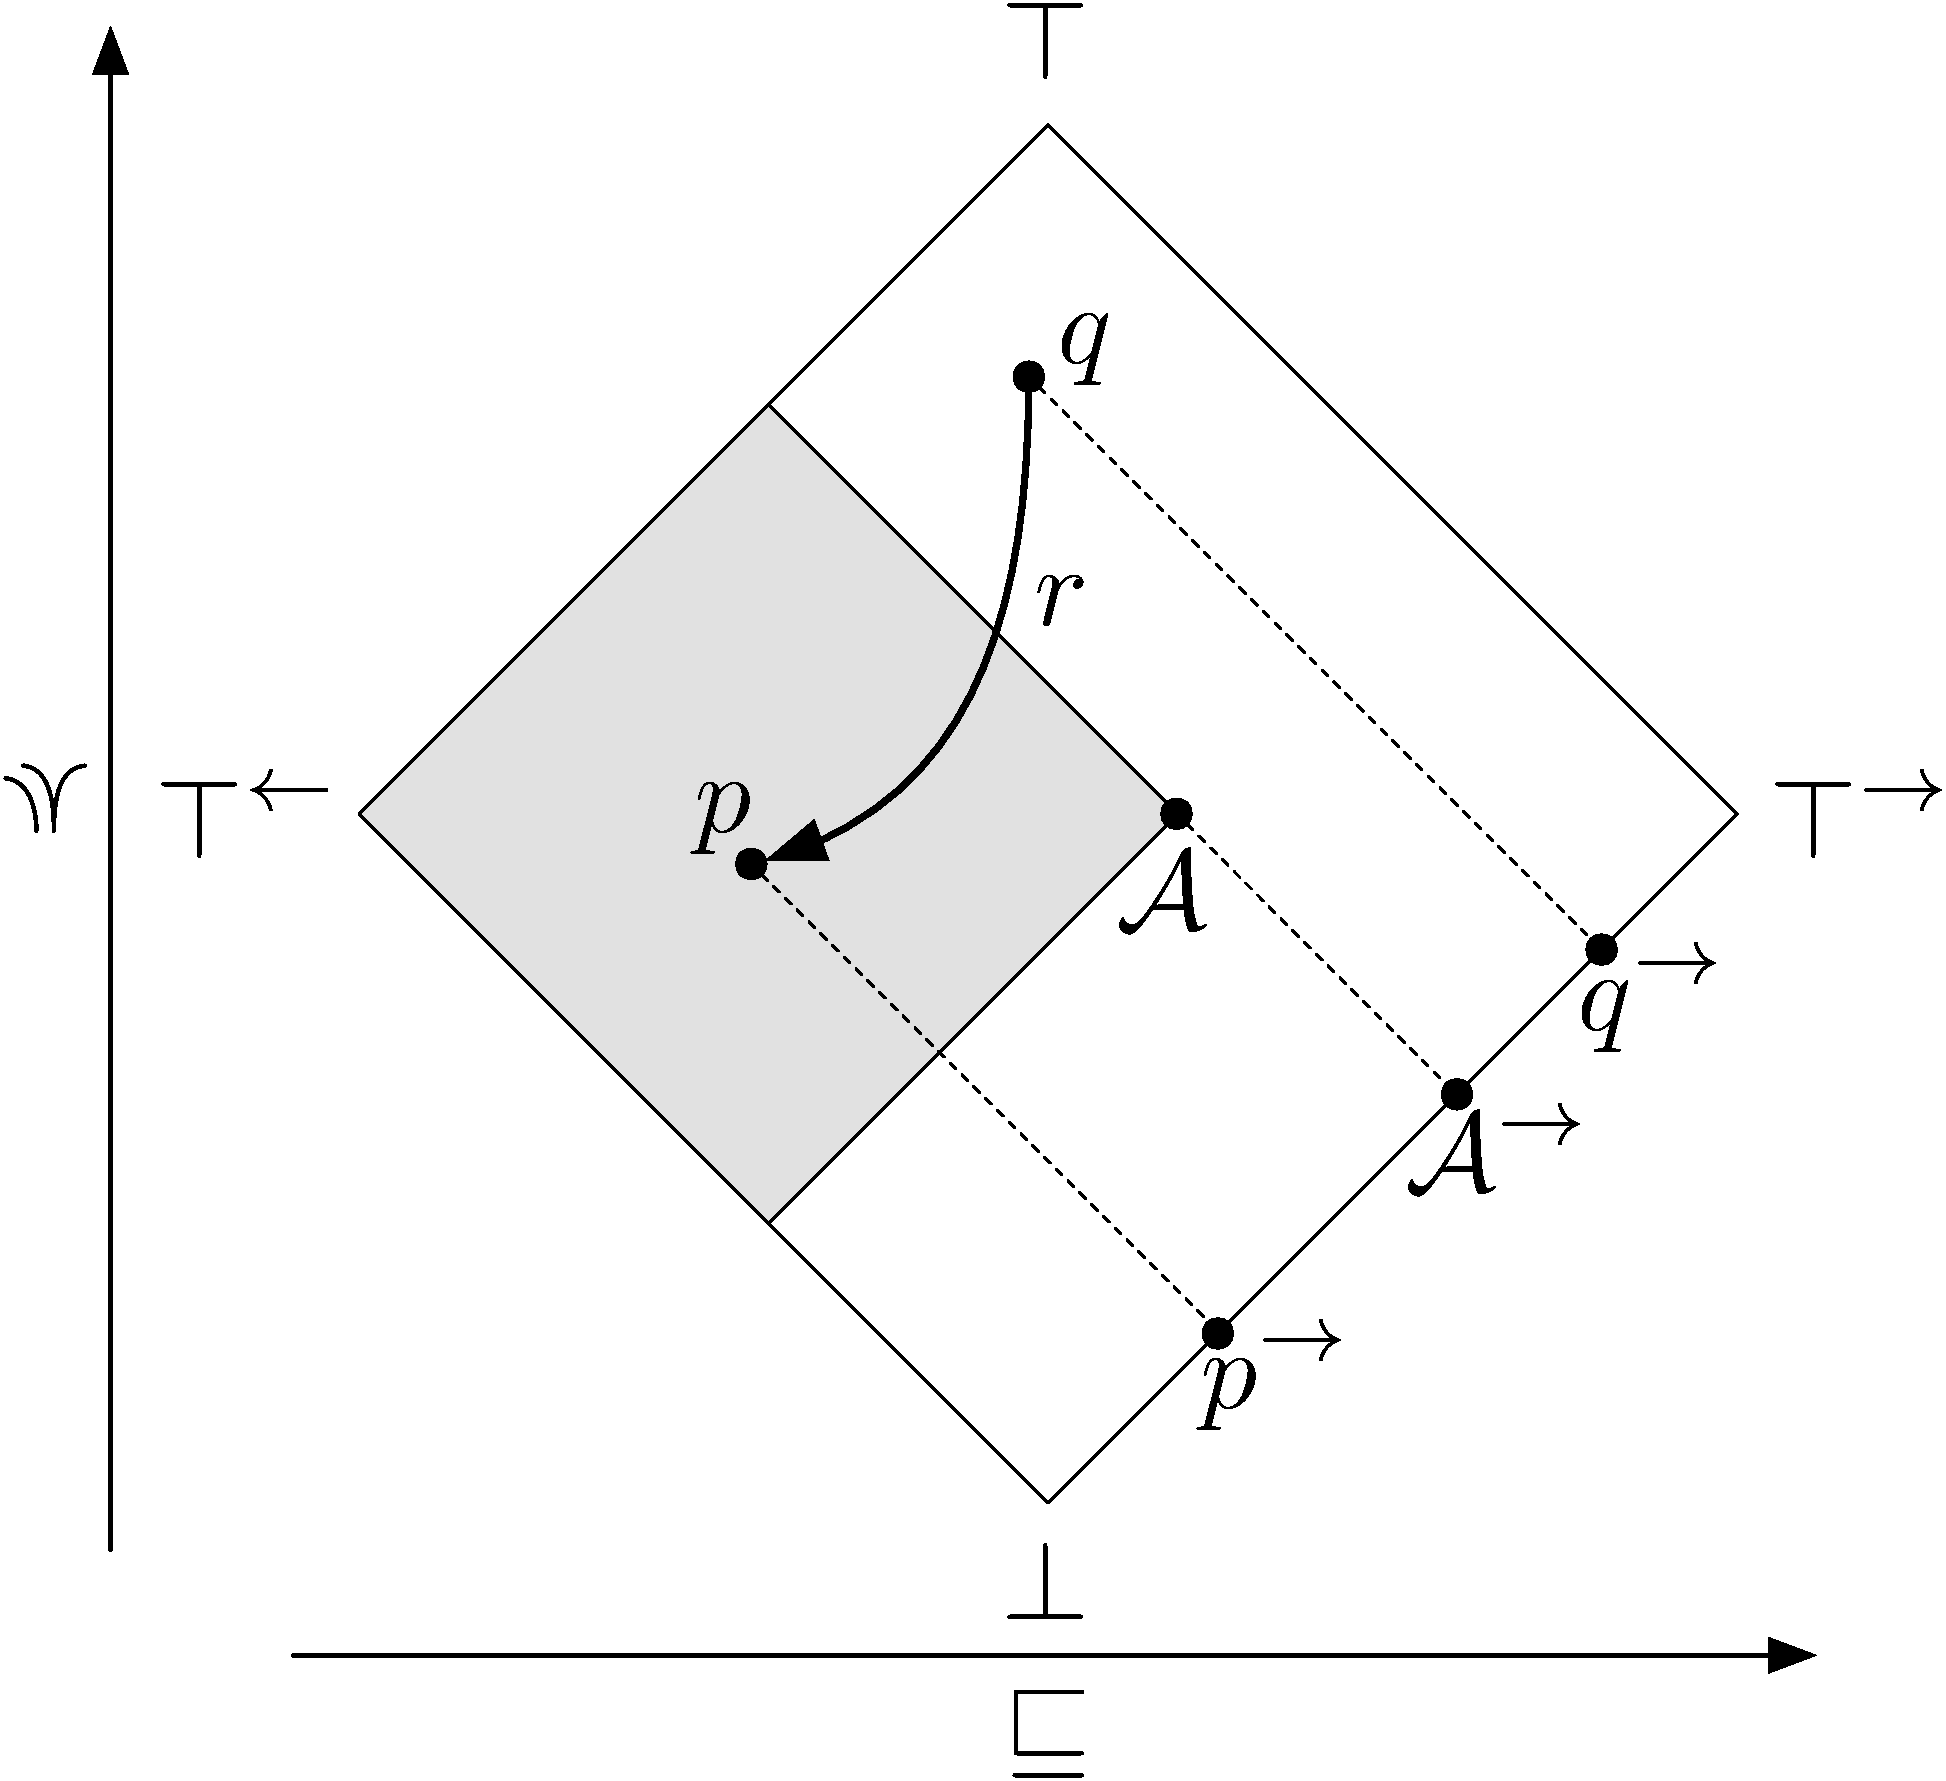
\includegraphics[scale=0.20]{Illustrations/bad-flow.pdf}
\end{minipage}%
\begin{minipage}{0.22\textwidth}
\caption{Information labeled as $q$, which previously could not be relabeled as $\Attacker$, can now be relabeled as $p$. This can, in turn, now be relabeled as $\Attacker$}\label{fig:bad-release}
\end{minipage}
\end{figure}

\paragraph{$\Attacker$-equivalence}
We define an $\Attacker$-equivalence relation that makes explicit which traces and stores an attacker $\Attacker$ can distinguish. As both traces and stores contain expressions, we define an $\Attacker$-equivalence on expressions, and Figure~\ref{fig:low-eq-expr} shows an excerpt of this. Rule \ruleref{Eq-High} states that any two expressions are $\Attacker$-equivalent in an environment with a current label that does not flow to the attacker. This idea is similar to the term erasure technique \cite{SRMMlio} and subsequent presentations of the LIO attacker model \cite{Stefan:2012:ACT:2364527.2364557, 10.1007/978-3-642-40203-6_40, 10.1007/978-3-319-24858-5_13}.

For most cases this judgment recursively inspects the subexpressions of each expression, but differ in a few cases: To relate dynamically allocated locations we use a partial bijection \cite{Banerjee:2002:SIF:794201.795164, Rajani2018} $\bijection: \Addr \partialto \Addr$ in \ruleref{Eq-Addr}. The most important rules are \ruleref{Eq-Labeled-1} that makes explicit the notion that an attacker cannot distinguish two terms labeled with a principal which does not flow to the attacker, and \ruleref{Eq-Labeled-2} which states that an attacker can ``look inside'' terms labeled with principals that flow to the attacker. When $\bijection$ is not important we write $\loweq{C}{\Attacker}{\expr_1}{\expr_2}$ to mean $\loweq{C}{\Attacker}[\bijection]{\expr_1}{\expr_2}$ for some bijection $\bijection$, where $C$ abbreviates $n; \env^1; \env^2$.

\begin{figure}
    \centering
    \begin{mathpar}
    \inferrule[Eq-High]{\nopostnotflowstoquery{C_i}{\env^i_n.\lblkw}{\Attacker}, i = 1,2}{\loweq{C}{\Attacker}[\bijection]{\expr_1}{\expr_2}}
    \and
    \inferrule[Eq-Low]{\nopostflowstoquery{C_i}{\env^i_n.\lblkw}{\Attacker}, i = 1,2 \\\\ \loweql{C}{\Attacker}[\bijection]{\expr_1}{\expr_2}}{\loweq{C}{\Attacker}{\expr_1}{\expr_2}}
    \and
    \inferrule[Eq-Addr]{\bijection(\addr_1) = \addr_2}{\loweql{C}{\Attacker}[\bijection]{\addr_1}{\addr_2}}
    \and
    \inferrule[Eq-Labeled-1]{\nopostnotflowstoquery{C_i}{p_i}{\Attacker}\quad i = 1,2}{\loweql{C}{\Attacker}[\bijection]{\lb{p_1}{\expr_1}}{\lb{p_2}{\expr_2}}}
    \and
    \inferrule[Eq-Labeled-2]{\nopostflowstoquery{C_i}{q}{\Attacker} \quad i = 1,2 \and \loweql{n; \env^1; \env^2}{\Attacker}[\bijection]{\expr_1}{\expr_2}}{\loweql{C}{\Attacker}[\bijection]{\lb{q}{\expr_1}}{\lb{q}{\expr_2}}}
    \end{mathpar}
    \caption{$\Attacker$-equivalence for terms and expressions. The meta-variable $C$ abbreviates $n; \env^1; \env^2$, and $C_i = n; \env^i$.}
    \label{fig:low-eq-expr}
\end{figure}

The $\Attacker$-equivalence relation on expressions induces an $\Attacker$-equivalence relation on events, and $\Attacker$-equivalence of traces are defined as pairwise $\Attacker$-equivalence of the events in the trace. We write $t_1 \simeq_{\Attacker}^{\bijection} t_2$ for the $\Attacker$-equivalence relation on traces, and $t_1 \simeq_{\Attacker} t_2$ to mean $t_1 \simeq_{\Attacker}^{\bijection} t_2$ for some bijection $\bijection$.

Finally, Figure~\ref{fig:low-eq-memories} shows $\Attacker$-equivalence on stores. Rule \ruleref{Store-Eq-Empty} states that two empty stores are $\Attacker$-equivalent, and rule \ruleref{Store-Eq-Low} states that extending two stores with $\Attacker$-equivalent expressions preserves $\Attacker$-equivalence. Lastly, rules \ruleref{Store-Eq-High-1} and \ruleref{Store-Eq-High-2} states that both stores can be extended with terms labeled with a principal that does not flow to $\Attacker$ without the attacker being able to distinguish the stores. We extend the notion of $\Attacker$-equivalence on stores to $\Nameset$-indexed sets of stores and write $\loweq{C}{\Attacker}[\bijection]{\globalstore}{\altglobalstore}$ when $\forall n \in \Nameset~.~ \loweq{C}{\Attacker}[\bijection]{\globalstore(n)}{\altglobalstore(n)}$ where $C$ abbreviates $m; \env^1; \env^2$.

To simplify the statement of our end-to-end security guarantee note that, for any $n, m \in \Nameset$ we have $\loweq{n; \emptyenv; \emptyenv}{\Attacker}{\store}{\altstore}$ if and only if $\loweq{m; \emptyenv; \emptyenv}{\Attacker}{\store}{\altstore}$. Thus, we write $\store \simeq_{\Attacker} \altstore$ to mean $\loweq{n; \emptyenv; \emptyenv}{\Attacker}{\store}{\altstore}$ for some $n$.

\begin{figure}
    \centering
    \begin{mathpar}
    \inferrule[Store-Eq-Empty]{~}{\loweq{C}{\Attacker}[\bijection]{\varnothing}{\varnothing}}
    \and
    \inferrule[Store-Eq-Low]{\bijection(\addr_1) = \addr_2 \and \loweq{C}{\Attacker}[\bijection]{\expr_1}{\expr_2} \\\\ \nopostflowstoquery{C_i}{q}{\Attacker}\quad i = 1,2 \\\\ \loweq{C}{\Attacker}[\bijection]{\store_1}{\store_2} \\\\ \store_i' = \extend{\store_i}{\addr_i}{(\lb{q}{\expr_i})}}{\loweq{C}{\Attacker}[\bijection]{\store_1'}{\store_2'}}
    \and
    \inferrule[Store-Eq-High-1]{\nopostnotflowstoquery{C_1}{q}{\Attacker} \\\\ \loweq{C}{\Attacker}[\bijection]{\store_1}{\store_2}}{\loweq{C}{\Attacker}[\bijection]{\extend{\store_1}{\addr}{\lb{q}{\expr}}}{\store_2}}
    \and
    \inferrule[Store-Eq-High-2]{\nopostnotflowstoquery{C_2}{q}{\Attacker} \\\\ \loweq{C}{\Attacker}[\bijection]{\store_1}{\store_2}}{\loweq{C}{\Attacker}[\bijection]{\store_1}{\extend{\store_2}{\addr}{\lb{q}{\expr}}}}
    \end{mathpar}
    \caption{$\Attacker$-equivalence for stores. The meta-variable $C$ abbreviates $n; \env^1; \env^2$, and $C_i = n; \env^i$.}
    \label{fig:low-eq-memories}
\end{figure}

\paragraph{Attacker knowledge}
We present our noninterference result using the notion of attacker knowledge \cite{Askarov:2008:TNL:1462455.1462485, 4223226}. The attacker's knowledge is the set of initial stores that could lead to a given observable trace, and a larger knowledge correspond to more uncertainty about the initial memory. Formally, an attacker's knowledge given a trace $t$ produced by expression $\expr$ and the initial set of stores $\globalstore$ is the set
\begin{equation*}
k^n_{\Attacker}(\globalstore, \expr, t) = \left\{ \, \altglobalstore \, \middle\vert \, \globalstore \simeq_{\Attacker} \altglobalstore \wedge \, \gconfig{n}{\emptyenv}{S} \gstepstos[][\Attacker \filtertrace t'] \wedge \, t \simeq_{\Attacker} t' \, \right\}
\end{equation*}
where $S(m) = \config{\altglobalstore(n)}{\llbracket \expr \rrbracket_n(m)}$ and
\begin{equation*}
\llbracket \expr \rrbracket_n(m) =
\begin{cases}
\expr & \text{ if } n = m\\
\termsym & \text{ otherwise }
\end{cases}
\end{equation*}
ensures that expression $\expr$ is initially evaluated on node $n$, and the remaining nodes start off with an empty list of expressions.

As is standard for termination-insensitive noninterference (TINI) the policy \cite{6234468} is defined as all possible terminating stores
\begin{equation*}
k^n_{\Attacker}(\globalstore, \expr) = \left\{ \,\altglobalstore \, \middle\vert \, \globalstore \simeq_{\Attacker} \altglobalstore \wedge \, \gconfig{n}{\emptyenv}{S} \gstepstos \, \right\}
\end{equation*}
where $S(m) = \config{\altglobalstore(n)}{\llbracket \expr \rrbracket_n(m)}$. We can now state TINI for \lang{} as follows.

\begin{theorem}[Noninterference]\label{thm:ni}
Let $\expr$ satisfy $\hastype{n; \tenv}{\expr}{\type}$.
If $\gconfig{n}{\varnothing}{S} \gstepstos[][\Attacker \filtertrace t]$ for $S(m) = \config{\globalstore(m)}{\llbracket \expr \rrbracket_n(m)}$ such that $\good{\Attacker}{t}$ then $k^n_{\Attacker}(\globalstore, \expr, t) \supseteq k^n_{\Attacker}(\globalstore, \expr)$.
\end{theorem}

Theorem~\ref{thm:ni} is proved using a generalized version of the statement that quantifies over any two $\Attacker$-equivalent global configurations $\gconfig{n_1}{\env_1}{S_1}$, $\gconfig{n_2}{\env_2}{S_2}$ that proves they emit $\Attacker$-equivalent observable traces. An important invariant obtained by quantifying only over good traces is that whenever $\actsforquery{n; \env_1}{p}{q}{\level}$ and $\nopostflowstoquery{n; \env_1}{\level}{\Attacker}$ it holds that $\actsforquery{n; \env_2}{p}{q}{\level}$ and $\nopostflowstoquery{n; \env_2}{\level}{\Attacker}$. The technical report \cite{techreport} contains a complete proof of Theorem~\ref{thm:ni}.

As seen in \ruleref{E-Get-Label} in Figure~\ref{fig:monadic-reductions}, the current label is public information. Thus, one might wonder if it is possible to raise the current label depending on information that should not flow to an attacker - perhaps by some clever trust checking that unlabels different delegations in two different (but $\Attacker$-equivalent) executions. However, as Theorem~\ref{thm:ni} shows, an attacker cannot learn any information by inspecting the current label.